\documentclass[border=6pt]{standalone}
\usepackage[T1]{fontenc}
\usepackage{courier}
\usepackage[scaled=0.95]{helvet}
\renewcommand{\familydefault}{\sfdefault}
\usepackage{sfmath}
\usepackage[version=4]{mhchem}
\usepackage{tikz}
\usepackage{pgfplots}
\pgfplotsset{compat=newest}
\usetikzlibrary{arrows.meta,positioning,calc,fit,backgrounds,shapes.geometric,decorations.pathreplacing,patterns}
\definecolor{ink}{HTML}{17233A}
\definecolor{inksoft}{HTML}{44506A}
\definecolor{teal}{HTML}{0E6B6B}
\definecolor{tealsoft}{HTML}{E5F0EF}
\definecolor{amber}{HTML}{B26B12}
\definecolor{ambersoft}{HTML}{FBF0DF}
\definecolor{blue}{HTML}{2F6690}
\definecolor{bluesoft}{HTML}{E3ECF4}
\definecolor{plum}{HTML}{7A4D8C}
\definecolor{plumsoft}{HTML}{EFE7F3}
\definecolor{greyc}{HTML}{8A94A3}
\definecolor{linec}{HTML}{D3DCE1}
\definecolor{oxy}{HTML}{C0392B}
\definecolor{carb}{HTML}{3B4252}
\definecolor{hyd}{HTML}{E6E9EE}
\definecolor{nit}{HTML}{2F6690}
\tikzset{
  every picture/.style={line cap=round,line join=round},
  lab/.style={font=\small, text=inksoft},
  >={Stealth[length=7pt]},
}
\pgfplotsset{
  every axis/.append style={axis line style={inksoft}, tick style={inksoft}, tick label style={font=\footnotesize, text=inksoft}, label style={font=\small, text=ink}},
}
% fragment tile: \frag{node name}{position}{colour}{content}
\newcommand{\frag}[4]{\node[draw=#3, fill=#3!12, line width=1.4pt, rounded corners=6pt, minimum width=1.25cm, minimum height=1.05cm, text=#3, font=\bfseries] (#1) at (#2) {#4};}
\newcommand{\ring}{\tikz[baseline=-0.6ex]{\draw[line width=1.1pt] (0:0.3)--(60:0.3)--(120:0.3)--(180:0.3)--(240:0.3)--(300:0.3)--cycle; \draw[line width=0.8pt] (0,0) circle (0.16);}}
\newcommand{\bond}[2]{\draw[ink, line width=2.2pt] (#1) -- (#2);}

\begin{document}
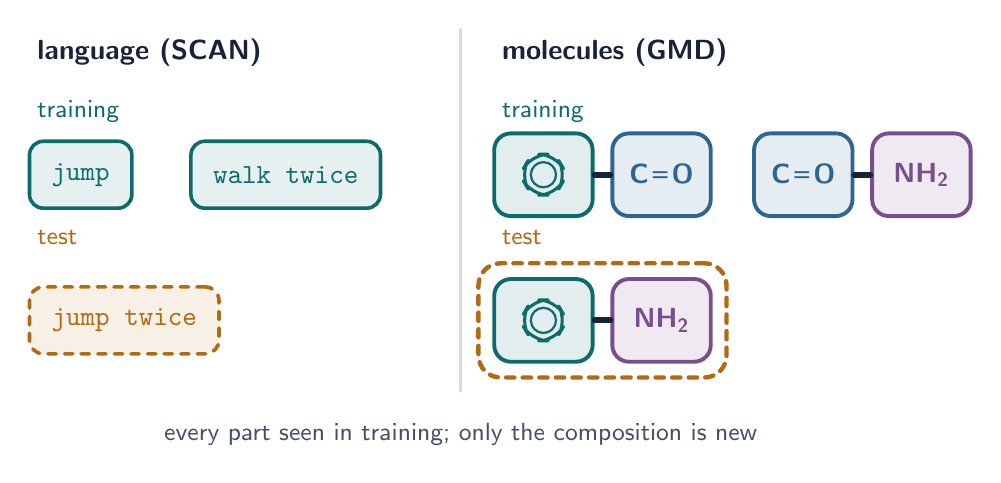
\begin{tikzpicture}[cmd/.style={draw=#1, fill=#1!10, line width=1.3pt, rounded corners=5pt, font=\ttfamily\bfseries, text=#1, minimum height=0.85cm, inner xsep=8pt}]
\node[font=\bfseries, text=ink, anchor=west] at (-0.3,4.1) {language (SCAN)};
\node[font=\small, text=teal, anchor=west] at (-0.3,3.35) {training};
\node[cmd=teal, anchor=west] at (-0.3,2.55) {jump};
\node[cmd=teal, anchor=west] at (1.75,2.55) {walk twice};
\node[font=\small, text=amber, anchor=west] at (-0.3,1.75) {test};
\node[cmd=amber, anchor=west, dashed] at (-0.3,0.7) {jump twice};
\draw[linec, line width=1pt] (5.2,-0.2) -- (5.2,4.4);
\node[font=\bfseries, text=ink, anchor=west] at (5.6,4.1) {molecules (GMD)};
\node[font=\small, text=teal, anchor=west] at (5.6,3.35) {training};
\frag{a1}{6.25,2.55}{teal}{\ring}\frag{b1}{7.75,2.55}{blue}{\ce{C=O}}\bond{a1}{b1}\frag{b2}{9.55,2.55}{blue}{\ce{C=O}}\frag{c2}{11.05,2.55}{plum}{\ce{NH2}}\bond{b2}{c2}
\node[font=\small, text=amber, anchor=west] at (5.6,1.75) {test};
\frag{a3}{6.25,0.7}{teal}{\ring}\frag{c3}{7.75,0.7}{plum}{\ce{NH2}}\bond{a3}{c3}
\node[draw=amber, line width=1.6pt, dashed, rounded corners=8pt, fit=(a3)(c3), inner sep=5pt] {};
\node[font=\small, text=inksoft, align=center] at (5.2,-0.75) {every part seen in training; only the composition is new};
\end{tikzpicture}
\end{document}
